
The claimed trivialization of $AK(3)$ in \cite{shehper2024makesmathproblemshard} comes from demonstrating that $AK(3)$ is stably AC-equivalent to the following presentation from \cite{myasnikov2003andrewscurtisequivalence}:
\[
MMS3 := \langle x,y,z \,\, \mid \,\, x=z\cdot [[y^{-1},x^{-1}],z], y=x\cdot [[y^{-1},x^{-1}],z^{-1}]\cdot [z^{-1},x], x^{-1}yz\rangle.
\] 
The presentation $MMS3$ was believed to be stably AC-trivial because the first two relations were thought to be obtained from the Wirtinger presentation of the unknot in Figure~\ref{fig:unknot} from \cite{myasnikov2003andrewscurtisequivalence}. In \cite{myasnikov2003andrewscurtisequivalence}, the following purported presentation is given as the Wirtinger presentation of the unknot:
\[
\begin{aligned}
WWU=\left\langle x_1, x_2, x_3, x_4, x_5, x_6, x_7, x_8, x_9, x_{10}, x_{11}, x_{12}, x_{13}, x_{14} \right. \mid\, &x_1=x_{10} x_{14} x_{10}^{-1}, x_2=x_{10}^{-1} x_1 x_{10},\\
&x_3=x_1^{-1} x_2 x_1, x_4=x_6^{-1} x_3 x_6,\\
&x_5=x_{12} x_4 x_{12}^{-1},x_6=x_7^{-1} x_5 x_7, \\
&x_7=x_4^{-1} x_6 x_4, x_8= x_1 x_7 x_1^{-1}, \\
&x_9=x_{11}^{-1} x_8 x_{11}, x_{10}=x_{14} x_9 x_{14}^{-1} \\
&x_{11}=x_2^{-1} x_{10} x_2, x_{12}=x_1^{-1} x_{11} x_1 \\
& x_{13}=x_5 x_{12} x_5^{-1}, x_{14}=x_1 x_{13} x_1^{-1}\left. \right\rangle
\end{aligned}
\]

We obtain $MMS3$ after deleting the relation $x_{12}=x_1^{-1}x_{11}x_{1}$ and adding the relation $w=x^{-1}yz$, and then using substitution to simplify the presentation. 

Unfortunately, $WWU$ is not the Wirtinger presentation of the unknot in Figure~\ref{fig:unknot}. The error is that the relation $x_{13}=x_5 x_{12} x_5^{-1}$ is incorrect; it should instead be $x_{13}=x_4 x_{12} x_4^{-1}$. Indeed $WWU$ is not the Wirtinger presentation of any knot: in a Wirtinger presentation, any one relator is redundant, so a Wirtinger presentation with any relator removed is a presentation of the knot group—in the case an unknot, the infinite cyclic group $\mathbb{Z}$. Yet removing different relators from $WWU$ gives different groups. For example, if $x_7=x_4^{-1} x_6 x_4$ is eliminated, then the resulting group is the three-stand braid group, whereas if the relator $x_{14}=x_1 x_{13} x_1^{-1}$ is removed, we get $\mathbb{Z}$. Most importantly, however, the presentation $WWU$ with the relator $x_{12}=x_1^{-1}x_{11}x_1$ removed—the choice made in \cite{myasnikov2003andrewscurtisequivalence} that leads to $MMS3$—is not a presentation of $\mathbb{Z}$. 

Because of these facts, we cannot use Reidemeister moves to show the stable AC-triviality of $MMS3$ and therefore $AK(3)$ as well.  

The following fact may be of interest: 
Let $MMU(w)$ be $WWU$ with the relator $x_7=x_4^{-1} x_6 x_4$ eliminated, and with the added relator $w$ to trivialize the group. Then we have the following proposition: 

% We can drive a balanced presentation $MMSU$ of the trivial group from $WWU$.  
% The presentation $MMSU$ is an interesting balanced presentation of the trivial group: if it would be stably Andres-Curtis trivial, then we will show that the whole sequence of $AK(n)$ will be stably AC-trivial.

\begin{myprop}  The balanced presentation $MMU(w)$ of the trivial group is stably AC-equivalent to $\langle x,y \mid xyx=yxy, w\rangle$; in particular, for $w_n=x^{-n}y^{n+1}$, we have that $MMU(w_n)$ is stably AC-equivalent to
    $AK(n)$ for each $n\geq 1$. 
\end{myprop}


\begin{proof}

Eliminating the relator $x_7=x_4^{-1} x_6 x_4$, we add any word $w$ in $x_7$ and $x_{13}$ which trivializes the group. Note such a word will have exponent sum $\pm 1$. We show that this presentation is stably AC-equivalent to $\langle x,y \mid xyx=yxy, w\rangle$ for $x=x_7$ and $y=x_{13}$.

To do this, we first substitute $x_1=x_{10} x_{14} x_{10}^{-1}$ into the second relator to get $x_2=x_{14}$ and then eliminate $x_2$. Next from the third relator we have $x_{14}=x_{1} x_{3} x_1^{-1}$ and we substitute this into the relator $x_{14}=x_1 x_{13} x_1^{-1}$ to get $x_3=x_{13}$, and we eliminate $x_3$. Moreover, since the eleventh relator now reads $x_{11}=x_2^{-1} x_{10} x_2$ we substitute $x_{10}=x_{14}x_9x_{14}^{-1}$ to get $x_{11}=x_9$ and from this $x_9=x_8$ from the ninth relator.  Our presentation now reads
\[ \begin{aligned} \langle x_1, x_4, x_5, x_6, x_7, x_8, x_{10}, x_{12}, x_{13}, x_{14} \mid \, & x_1= x_{10} x_{14} x_{10}^{-1}, x_{13}= x_1^{-1} x_{14} x_{1}, x_4= x_6^{-1} x_{13} x_{6},\\
& x_5= x_{12} x_{4} x_{12}^{-1},x_6= x_7^{-1} x_{5} x_{7},x_8= x_{1} x_{7} x_1^{-1}, \\
&x_{10}= x_{14} x_{8} x_{14}^{-1}, x_{12}= x_1^{-1} x_{8} x_{1},x_{13}= x_{5} x_{12} x_5^{-1}, w\rangle  \end{aligned} \]

Now we substitute $x_8=x_1 x_7 x_1^{-1}$ into $x_{12}=x_1^{-1} x_8 x_1$ to get $x_{12}=x_7$ and we eliminate $x_{12}$. This now gives $x_5=x_7 x_4 x_7^{-1}$ which we substitute into $x_6= x_7^{-1} x_{5} x_{7}$ to get $x_6=x_4$ and from this we get $x_4=x_{13}$. We then eliminate $x_6$ and $x_4$. What remains is 

\[ \begin{aligned} \langle x_1, x_5, x_7, x_8, x_{13}, x_{14}\mid\, & x_1= x_{10} x_{14} x_{10}^{-1},x_{13}=x_1^{-1} x_{14} x_{1},x_8= x_{1} x_{7} x_1^{-1},\\
&x_{10}= x_{14} x_{8} x_{14}^{-1},x_5= x_{7} x_{13} x_7^{-1}, x_{13}= x_{5} x_{7} x_5^{-1}, w \rangle \end{aligned} \] 

Now we substitute $x_{10} = x_{14}x_8 x_{14}^{-1}$ into the first relator and eliminate $x_{10}$, followed by substituting $x_{14}=x_{1} x_{13} x_1^{-1}$ and eliminating $x_{14}$. We next substitute $x_8=x_1 x_7 x_1^{-1}$ and eliminate $x_8$, and then $x_5=x_7 x_{13} x_{7}^{-1}$ and eliminate $x_5$. We are left with 
\[ \langle x_1, x_7, x_{13} \mid  x_7 x_{13} x_7 = x_{13} x_7 x_{13}, x_1 = x_{13} x_7 x_{13} x_7^{-1} x_{13}^{-1}, w  \rangle \] which, after setting $x=x_7, y=x_{13}$ is stably AC-equivalent to 
\[
\langle x,y \mid xyx=yxy, w\rangle.
\]

Thus by setting $w=x^{-n}y^{n+1}$, we obtain the proposition.

\end{proof}




\begin{figure}
    \centering
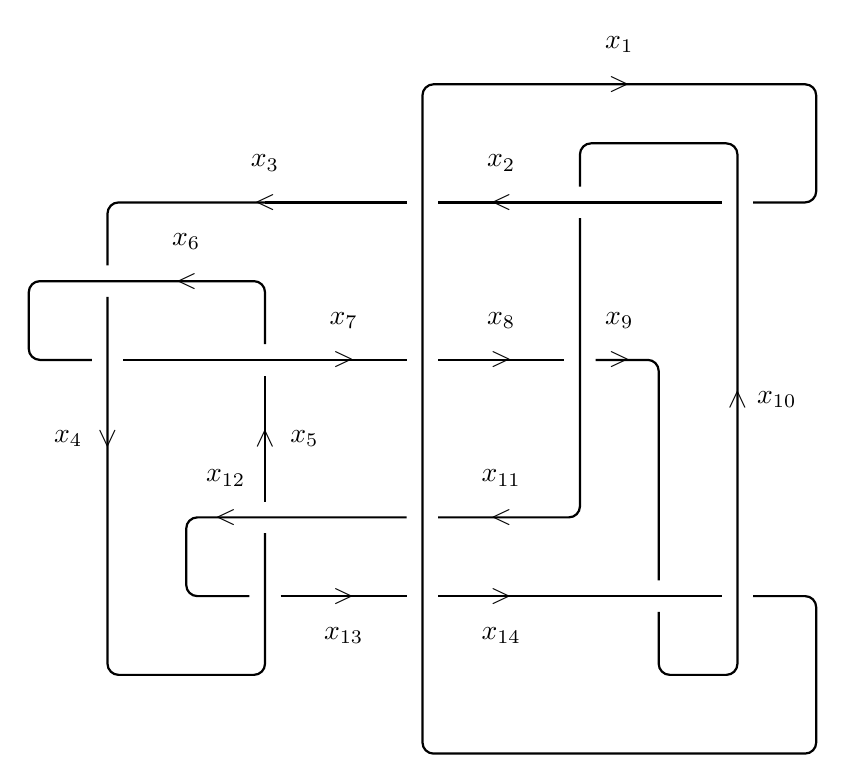
\begin{tikzpicture}
\draw[thick] (0,0)--(1.8,0);
%x3
\draw[thick] (2.2,0)--(5.8,0);
%x2
\draw[thick,rounded corners] (6.2,0)--(7,0)--(7,1.5)--(2,1.5)--(2,-7)--(7,-7)--(7,-5)--(6.2,-5);
%x1
\draw[thick,rounded corners] (0,0)--(-2,0)--(-2,-0.8);
%x3
\draw[thick,rounded corners] (-2,-1.2)--(-2,-6)--(0,-6)--(0,-4.2);
%x4
\draw[thick,rounded corners] (0,-3.8)--(0,-2.2);
%x5
\draw[thick,rounded corners] (0,-1.8)--(0,-1)--(-3,-1)--(-3,-2)--(-2.2,-2);
%x6
\draw[thick,rounded corners] (-1.8,-2)--(1.8,-2);
%x7
\draw[thick,rounded corners] (1.8,-4)--(-1,-4)--(-1,-5)--(-0.2,-5);
%x12
\draw[thick,rounded corners] (0.2,-5)--(1.8,-5);
%x13
\draw[thick,rounded corners] (2.2,-4)--(4,-4)--(4,-0.2);
%x11
\draw[thick,rounded corners] (4,0.2)--(4,0.75)--(6,0.75)--(6,-6)--(5,-6)--(5,-5.2);
%x10
\draw[thick,rounded corners] (2.2,-5)--(5.8,-5);
%x14
\draw[thick,rounded corners] (5,-4.8)--(5,-2)--(4.2,-2);
%x9
\draw[thick,rounded corners] (2.2,-2)--(3.8,-2);
%x8

\node at (4.5,1.5){$>$};
\node at (3,0){$<$};
\node at (0,0){$<$};
\node at (-2,-3){\rotatebox{90}{$<$}};
\node at (0,-3){\rotatebox{90}{$>$}};
\node at (-1,-1){$<$};
\node at (1,-2){$>$};
\node at (3,-2){$>$};
\node at (4.5,-2){$>$};
\node at (6,-2.5){\rotatebox{90}{$>$}};
\node at (3,-4){$<$};
\node at (-0.5,-4){$<$};
\node at (1,-5){$>$};
\node at (3,-5){$>$};

\node at (4.5,2){$x_1$};
\node at (3,0.5){$x_2$};
\node at (0,0.5){$x_3$};
\node at (-2.5,-3){$x_4$};
\node at (0.5,-3){$x_5$};
\node at (-1,-0.5){$x_6$};
\node at (1,-1.5){$x_7$};
\node at (3,-1.5){$x_8$};
\node at (4.5,-1.5){$x_9$};
\node at (6.5,-2.5){$x_{10}$};
\node at (3,-3.5){$x_{11}$};
\node at (-0.5,-3.5){$x_{12}$};
\node at (1,-5.5){$x_{13}$};
\node at (3,-5.5){$x_{14}$};


\end{tikzpicture}
    \caption{Unknot diagram}
    \label{fig:unknot}
\end{figure}